\section{Adversary Argumenter}%
\label{sec:adversaryargumenter}

\begin{frame}
	\frametitle{Pensum}
	\begin{itemize}
		\item Baase 3: \textbf{Adversary nedre grænse argumenter}
		\item Baase 3.5: \textbf{Adversary Median Problem}
		\item Jørgens noter: \textbf{Noter på nedre grænser}
		\item Weekly Note 12
		\item Video 24-25
	\end{itemize}
\end{frame}

\begin{frame}[allowframebreaks]
  \frametitle{Nedre Grænser for Sammenligningsbaseret Sortering}
  \begin{itemize}
	\item Vi vil gerne bevise at en algoritme mindst vil kunne lave $\Theta(n \log n)$ sammenligninger.
	\item Til at bevise dette bruger vi \textit{decision trees}.
	\item Alle deterministiske sammenligningsbaseret sorteringsalgoritmer $A$  kan associeres med et decision tree.
	\item Et decision tree har en knude som stiller en udtalelse op, e.g. $x_{14} < x_{17}$, og har så to kanter, en for hvis \textit{ja} og en for hvis \textit{nej}.
	\item Disse kanter fører så videre til flere knuder der også har nej/ja kanter, osv. indtil du kommer til bladene.
	\item Det vil også sige at roden af træet er den første sammenligning der bliver lavet.
	\item Hvert blad repræsenterer altså en permutation for hvordan tallene kan se ud.
	\item Det vil sige at alle mulige permutationer er blade, og dermed er der mindst $n!$ blade, for et input af størrelse $n$. Det er også muligt at en permutation kan være i et blad mere end én gang.
	\item Et decision træ er et binært træ, hvilket betyder at for hvert ``niveau'' i træet, bliver antallet af knuder \textbf{højest} fordoblet.
	\item Dermed er der også højest $2^{h}$ blade, hvor $h$ er højden på træet.
	\item Dermed må $2^{h} \ge n!$.
	\item Dermed må $h \ge \log n! \ge n \log n - cn$
	\item Vi får dette fra at $2^{h} \ge n!$, hvor vi kan tage $\log_{2}$ på begge sider og få $\log_{2}(2^{h}) \ge \log_{2}(n!)$ som giver $h \ge \log_{2}(n!)$.
	\item Den anden del, at $\log n! \ge n \log n - cn$ håber jeg ikke vi skal kunne til eksamen, for ChatGPT's bevis bruger både $\pi$ og $e$, og er i øvrigt ultra langt.
	\item Hver vej fra roden til et blad svarer til sammenligninger lavet af $A$ til at sortere et input. Dermed er antallet af sammenligninger lig med længden af vejen.
	\item Dermed bruger $A$ \textbf{mindst} $n \log n - cn$ sammenligninger på et input.
	\item Vi kan også finde en nedre grænse for den gennemsnitlige mængde af sammenligninger via decision trees.
	\item Givet en mængde $P$ som indeholder alle veje fra roden til bladene, kan vi definere $epl$ (externaexternal path length) til at være:
		  \begin{equation*}
			epl = \sum_{p \in P} \text{længde}(p)
		  \end{equation*}
	\item Lemma 2.8 i Baase, siger at $epl$ er minimeret når $T$ er ``almost balanced'', som vil sige at forskellen i distancen mellem rodden og alle blade enten er den samme for alle blade, eller er højest 1.
  \end{itemize}
  \begin{center}
	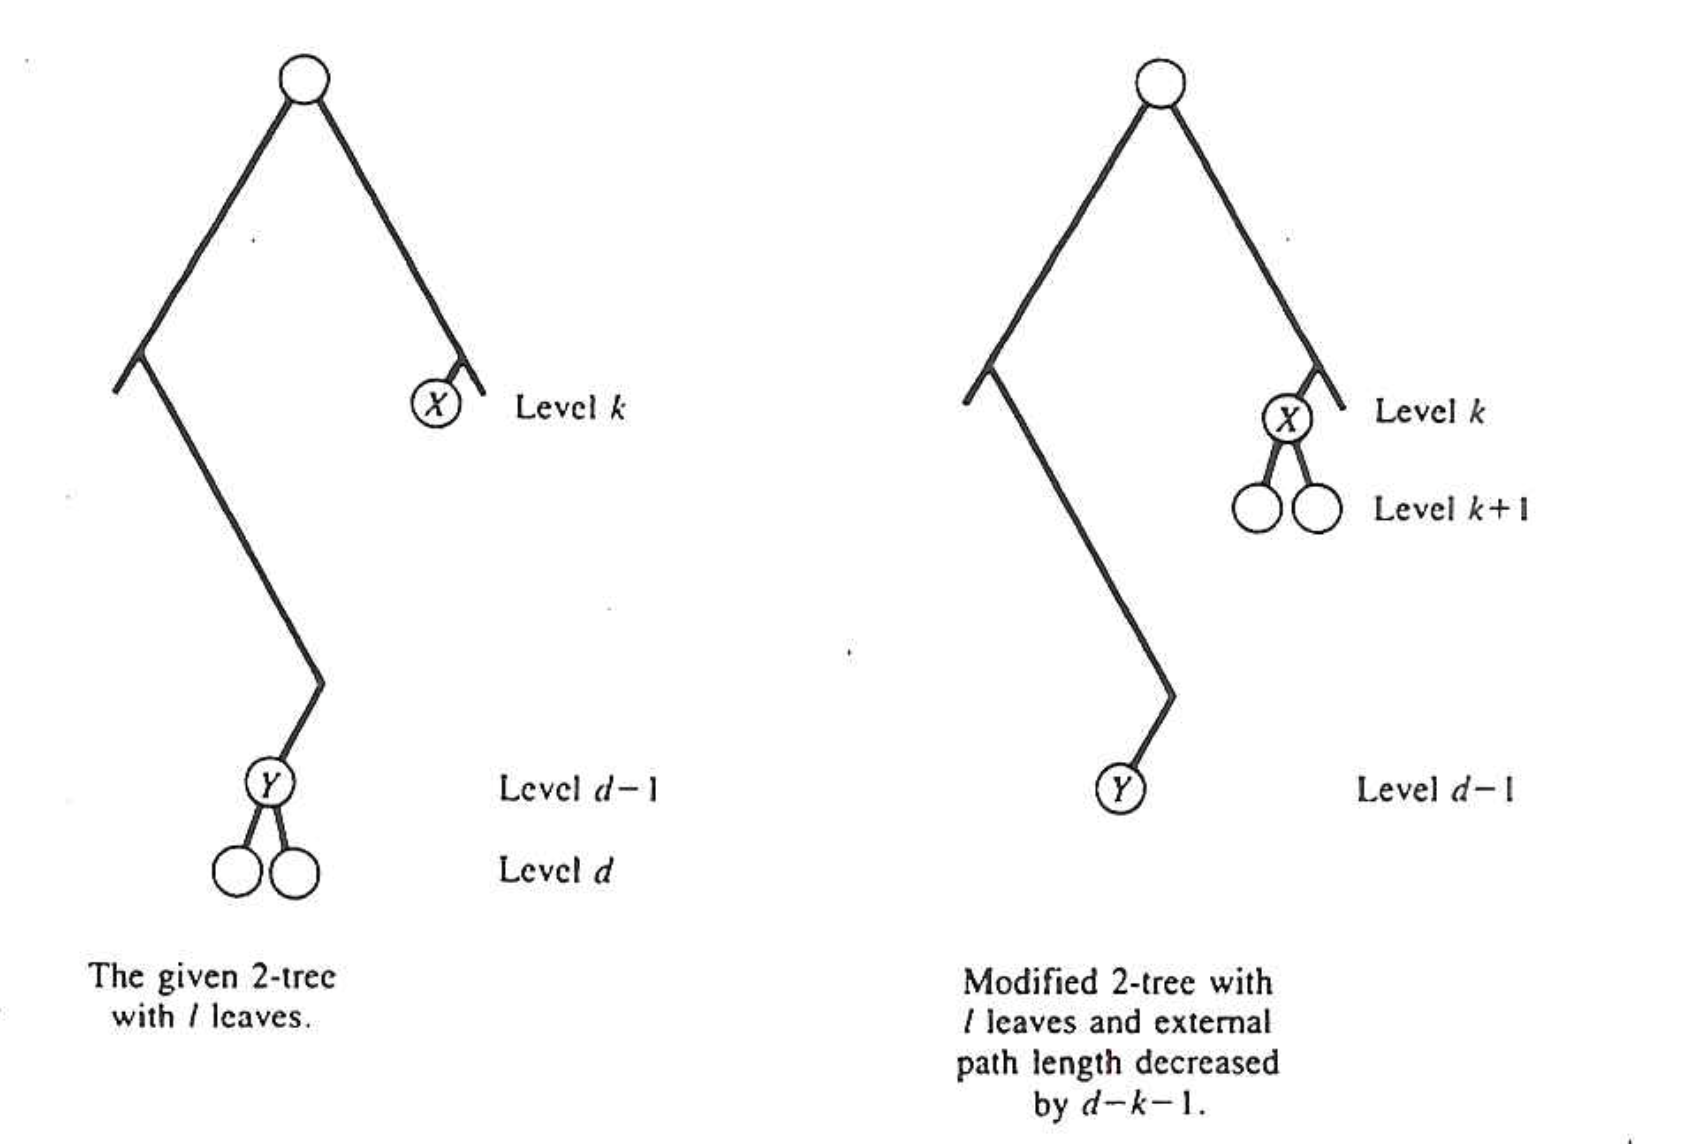
\includegraphics[scale=0.3]{figur/baaselemma28.png}
  \end{center}
  \begin{itemize}
	\item Beviset givet i Baase siger at hvis et blad $X$ på level $k \le d-2$, så kan vi lave et træ med det samme antal blade, og en mindre $epl$.
	\item  Vi vælger en knude $Y$ på level $d-1$, som ikke er et blad, og fjerner dens børn, og giver så to børn til $X$. Antallet af børn har ikke ændret sig.
	\item EPL-en er blevet nedsat med $2d+k$, fordi vejene til børnene (to børn, hver af længde $d$) af $Y$ og vejen til $X$ (længde $k$) ikke længere er forbundet.
	\item Når vi så tager børnene tilbage til $X$  så får vi en øgning i EPL-en. Da børnene til $X$ vil være på level $k+1$, og der er to, bliver det $2(k+1)$. Da $Y$ forbliver på level $d-1$ er længden $d-1$.
	\item Dermed er den totale øgning i EPL $2(k+1)+(d-1)=2k+2+d-1=2k+d+1$
	\item Vi vil nu gerne finde ændringen, som vi gør ved at fjerne øgningen fra aftagelsen.
	\item Aftagelsen: $2d+k$
	\item Øgningen: $2k+d+1$
	\item $(2d+k)-(2k+d+1) = 2d+k-2k-d-1=d-k-1$
	\item Vi ved at $k \le d-2$, så $d-k-1 > 0 $
	\item Så altså får vi et træ med en lavere EPL.
	\item Lemma 2.9: Minimums EPL-en for et decision træ med $l$ blade er $l \lfloor \log l \rfloor + 2(l-2^{\lfloor \log l\rfloor })$
	\item Hvis $l = 2^{k}$  for en $k$, og alle blade på level $\log l$, så er EPL--en $l \log l$
	\item Hvis $l \ne 2^{k}$ for en $k$, så er dybden af træet $d = \lceil \log l \rceil$ og alle bladene er på level $d-1$ og $d$.
	\item Summen for alle vejlængderne til niveau $d-1$ er $l(d-1)$.
	\item Alle blade på niveau $d$ skal altså tilføje $1$ ekstra til EPL--en.
	\item Antallet af blade på level $d$ er $2(l-2^{d-1})$, da, for hver knude på level $d-1$ som \textbf{ikke} er et blad, er der to blade på level $d$.
	\item Dermed er summen $l(d-1)+2(l-2^{d-1}) = l \lfloor \log l \rfloor + 2(l-2^{\lfloor \log l \rfloor})$.
	\item Grunden til at vi kan sige oprundet $\log l$, er fordi det er det nederste niveau, og $\log l$ vil give os en mellemting. Dermed er nedrundet det niveau der kommer over, e.g. 8 og 9, hvis $\log l = 8.4$. Vi kan kun forvente et heltal hvis $l = 2^{k}$.
	\item Bemærk at hvis $l = 2^{k}$ så vil $2(l-2^{k}) = 2(2^{k}-2^{k}) = 2(0) = 0$
	\item Lemma 2.10: Den gennemsnitlige længe af en vej i et 2-træ med $l$ blade er mindst $\lfloor \log l \rfloor$.
	\item Beviset her er ret nemt:
		  \begin{equation}
\frac{l \lfloor \log l \rfloor + 2(l-2^{\lfloor \log l \rfloor})}{l}  = \lfloor \log l\rfloor + \varepsilon
		  \end{equation}

	\item Hvor \(0 \le \varepsilon < 1\) da $l-2^{\lfloor \log l \rfloor }< \frac{l}{2}$, fordi $l > 2^{\lfloor \log l \rfloor}$
    \item Og $l$ kan højest være $2^{\lceil \log l \rceil} = 2^{\log l}$.
	\item Teorem 2.11: Den gennemsnitlige mængde af sammenligninger lavet af en algoritme til at sortere $n$ elementer er mindst $\lfloor \log n! \rfloor \approx \lfloor n \log n - 1.5n \rfloor$
  \end{itemize}
\end{frame}

\begin{frame}[allowframebreaks]
  \frametitle{Modstander Argumenter for Sortering}
\begin{itemize}
  \item Vores modstander til det her er ``incredibly powerful''.
  \item Vedkommende har en samling af permutationer af listen der skal sorteres, som opdateres efter et nyt valg er lavet i algoritmen.
  \item Dermed kan modstanderen, efter hvert skridt, finde den værst mulige permutation, som er mulig for algoritmen.
  \item Man kan se på en sorteringsalgoritme, som en algoritme der starter med at have alle $n!$ permutationer, og skal eleminere alle undtagen én som så bliver den sorteret permutation.
  \item Vi (Jørgen) introducerer følgende terminologi:
  \item \(\delta_{i}\) = permutationer der stadig er mulige efter den $i$'e sammenligning.
  \item Dermed er \(|\delta_{o}| = n!\)
  \item Hver gang din algoritme stiller spørgsmålet $x < y$? så er modstanderens mål er ``dræbe'' så få permutationer som muligt.
  \item Dermed vil modstanderen gerne svare således at $\frac{|\delta_{i}|}{|\delta_{i-1}|} \ge \frac{1}{2}$, altså at mere end halvdelen af permutationerne er tilbage.
  \item Det er ikke muligt at garantere mere end halvdelen, da det bedst mulige svar, ville fjerne halvdelen.
  \item Dermed skal du bruge \textbf{mindst} $\log_{2}n!$ sammenligninger før $|\delta_{k}|=1$.
  \item Vi viste tidligere at $\log_{2}n! = n \log n - cn$.
  \item De tidligere problemer vi har kigget på har det været nemt for modstanderen at finde et godt modsvar, men her kræver det utroligt meget for modstanderen.
\end{itemize}
\end{frame}
% 21:31 eller iindtil han er blevet færdig med at forklare det'' `nemme argument``''`.

\begin{frame}[allowframebreaks]
  \frametitle{Jørgens Argument}
 \begin{itemize}
   \item Jørgen har selv fundet på det her argument, men han fandt ud af at han ikke var den første til det:(
   \item Problemet med vores tidligere argument, er at det kræver for modstanderen at konstruere $\delta_{i}$ ud fra \(\delta_{i-1}\) hvilket kræver tid i forhold til \(|\delta_{i-1}|\).
   \item Jørgens modstander er langt mindre kraftfuld, og viser en nedre grænse på $\frac{1}{5}n \log n$ sammenligninger.
   \item Vi antager at $n = 2^{k}$.
   \item Vi kører på en træstruktur.
   \item Roden af træet har størrelse $n = 2^{k}$
   \item Da det er et binært træ, splitter dette op til 2 knuder (som han kalder bags).
   \item På niveau 1, (hvor roden er niveau 0) har vi så 2 knuder, som hver har $n/2 = 2^{k-1}$ størrelse.
   \item Dette fortsætter indtil niveau $l$ som har $n/2^{l} = 2^{k-l}$ størrelse, og $2^{l}$ knuder (bags).
   \item Jørgen forklarer det lidt snørklet, men jeg tror at ved niveau $l$ er $l = k$ og dermed er der en knude for hvert element.
   \item Når vi spørger $x < y$ så ``filtrerer'' vi dem ned til børnene af knuden, der spørges ind til.
   \item Du er først færdig med at sortere når \textbf{alle} elementer har været hele træet igennem, og er nede ved niveau $l$.
   \item Så hvis vi spørger $u < v?$ og modstanderen siger $u < v$. Så tager vi $u$ i ``posen'' til venstre, og $v$ i posen til højre.
   \item Måden modstanderen vælger at svare på, er ved at associere en tilstand til hver pose $b$ på niveau $l$. Der er tre tilstande:
   \item $b$ er \textbf{åbent}:
         \begin{itemize}
           \item Hver af de venstre og højre deltræer af $b$ har mindre end $2^{k-l-1}$ elementer.
         \end{itemize}
   \item $b$ er ``venstre-flushed'':
         \begin{itemize}
           \item Det venstre deltræ af $b$ har $2^{k-l-1}$ elementer.
         \end{itemize}
   \item $b$ er ``højre-flushed'':
         \begin{itemize}
           \item Det højre deltræ af $b$ har  $2^{k-l-1}$ elementer.
         \end{itemize}
   \item Husk at der i alt er $2^{l}$ elementer, så dermed vil hver bag i gennemsnit kunne tage $2^{k-l}$ elementer. Da hvert deltræ har under $2^{k-l-1}$ elementer, betyder det at gennemsnittet ikke er nået endnu.
   \item Du kan altså se det som, at ``x-flushed'' betyder at $\overline{x}$ har plads til at tage flere elementer, men $x$ har ikke.
   \item Vi kigger på algoritmerne i Jørgens \href{https://imada.sdu.dk/u/jbj/DM553/Slides21/Lect24.pdf}{noter} side 7.
   \item Nu til strategien som modstander.
   \item Når algoritmen $A$ spørger om $x < y$, så vælger modstanderen at flytte 2, 1, eller nul elementer ned til et deltræ, dog med en undtagelse: hvis en af børnene er fyldte, så flytter vi alle andre elementer ned til det andet barn.
   \item Vi kigger igen på Jørgens noter, denne gang side 8.
   \item MANGLER: Bevis for $\Omega(n \log n)$.
 \end{itemize}
\end{frame}

%%% Local Variables:
%%% mode: latex
%%% TeX-engine: xetex
%%% TeX-command-extra-options: "-shell-escape"
%%% TeX-master: "main"
%%% End:
